\subsection{ELISE Projektbeschreibung} \label{elise-subsec}

\todo[inline,color=green!40]{RfP}


ELISE ist ein Verbundprojekt, welches die Entwicklung eines interaktives und emotionssensitiven Lernsystems zur Kompetenzentwicklung im Bereich der Gesch{\"a}ftsprozessmanagement plant. 
Hierf{\"u}r kamen f{\"u}nf Partner des Forschungskollegs (FoKoS) der Universit{\"a}t Siegen zusammen – der Lehrstuhl f{\"u}r Wirtschaftsinformatik \& Center for Responsible Innovation \& Design, die Forschungsgruppe Research Group for Pattern Recognition, der Lehrstuhl Medizinische Informatik und Mikrosystementwurf der Universit{\"a}t Siegen, der Spieleentwickler Limbic Entertainment GmbH und der Softwarehersteller Software AG. 
Zusammen befassen sie sich mit einem interaktiven und emotionssensitiven Lernsystems in Form eines Spiels, das in einer virtuellen Umgebung erfolgt. 
Zudem befasst sich das Projekt mit der Auswirkung von solcher Systeme hinsichtlich ethischer und gesellschaftlicher Aspekte auf die Akzeptanz potenzieller Nutzerinnen und Nutzer.
Abbildung \ref{fig-elise} zeigt das vorhaben, welches durch das Projekt Elise verwirklicht werden soll.


\begin{figure}[H] \centering
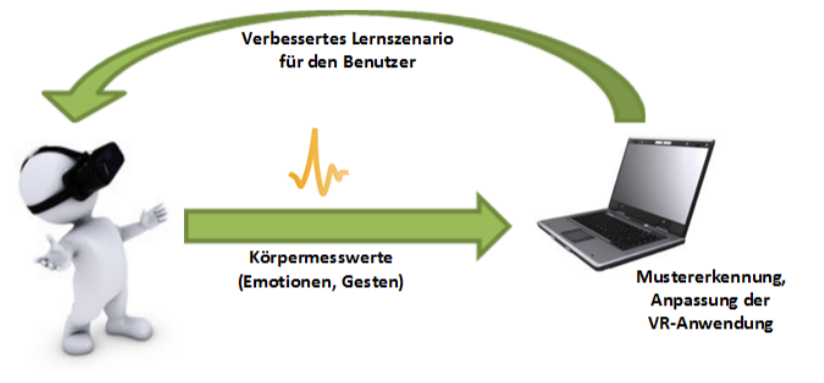
\includegraphics[width=12cm]{Images/elise_projektbeschreibung.png} 
\vspace{-0.3cm} 
\caption{Grobe {\"U}bersicht des Gesamtprojekts\cite{msckroenert}.}
\label{fig-elise} 
\end{figure}

Der Lehrstuhl Medizinische Informatik und Mikrosystementwurf entwickelt im Rahmen des Gesamtprojektes ein Sensorsystem, welches die Vital-, Elektroenzephalografie-, Elektrookulografie- und galavanische Hautreaktionwerte aufzeichnet. 
Diese werden dann vom Lehrstuhl f{\"u}r Mustererkennung ausgewertet. 
Die Lerninhalte der Hauptanwendung des ELISE-Projekts werden daraufhin an Emotionen und Gem{\"u}tslagen der Lernenden wie Gl{\"u}ck, Langeweile, Frustration auf Basis von biomedizinischer Daten angepasst, um so den individuellen Erfolg des Lernenden zu erh{\"o}hen.